\documentclass[Física - Práctica.root.tex]{subfiles}

\begin{document}

\section{Unidad 2}

\begin{enumerate}
  \item Un niño de \SI{21,0}{\kilogram} de peso se sienta en un subibaja a \SI{2,00}{\meter} del centro de giro. ¿Qué tan lejos del centro de giro deberá sentarse, del otro lado, su padre de \SI{105}{\kilogram} para que el balancín esté en equilibrio?

        \begin{multicols}{2}
          \begin{center}
            \begin{tikzpicture}
              \draw (-3,0) -- (3,0);
              \fill[green] (0,0) circle(2pt);
              \draw[->, red] (-2.5,1) node[anchor=south]{$F_n$} -- ++(0,-1);
              \draw[->, red] (2.5,1) node[anchor=south]{$F_p$} -- ++(0,-1);
              \draw[blue] (-1.25,0) node[anchor=north]{\SI{2,00}{\meter}};
              \draw[blue] (1.25,0) node[anchor=north]{$x$};
            \end{tikzpicture}
          \end{center}

          \[
            F_n=\SI{21,0}{\kilogram}\times\SI{9,80}{\meter\over\second\squared}
            =\SI{205}{\newton}
          \]
          \[
            F_p=\SI{105}{\kilogram}\times\SI{9,80}{\meter\over\second\squared}
            =\SI{1020}{\newton}
          \]
          \[
            \tau_n=rF_n\sin{\theta}
            =\SI{2,00}{\meter}\times\SI{205}{\newton}\times\sin{\ang{90}}
            =\SI{410}{\meter\newton}
          \]
          \[\tau_p=-\tau_n=\SI{-410}{\meter\newton}\]

          \[\SI{-410}{\meter\newton}=x\SI{1020}{\newton}\sin{\ang{-90}}\]
          \[\SI{-410}{\meter\newton}=x\times\SI{-1020}{\newton}\]
          \[\frac{\SI{-410}{\meter\newton}}{\SI{-1020}{\newton}}=x\]
          \[x=\boxed{\SI{0.402}{\meter}}\]
        \end{multicols}

  \item Un pintor de \SI{75,0}{\kilogram} pinta una pared estando de pie sobre una tabla larga que descansa apoyada en dos puntos sobre un andamio, tal como lo muestra la figura. Si la tabla es homogénea y tiene una masa de \SI{15,0}{\kilogram}, ¿cuán cerca del extremo izquierdo de la tabla podrá pararse sin que la tabla se incline?

        \begin{multicols}{2}
          \begin{center}
            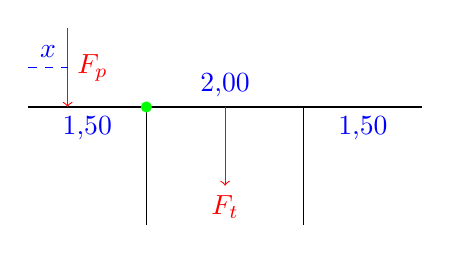
\begin{tikzpicture}
              \draw (-2.5,0) -- node[blue,anchor=north,pos=.5]{\SI{1,50}{\meter}} ++(1.5,0) coordinate(a) -- node[blue,anchor=south,pos=.5]{\SI{2,00}{\meter}} ++(2,0) coordinate(b) -- node[blue,anchor=north,pos=.5]{\SI{1,50}{\meter}} ++(1.5,0);
              \draw (a) -- ++(0,-1.5);
              \draw (b) -- ++(0,-1.5);
              \fill[green] (a) circle(2pt);
              \draw[->, red] ++(-2,1) -- ++(0,-1) node[pos=.5,anchor=west]{$F_p$};
              \draw[dashed, blue] (-2.5,.5) -- (-2,.5) node[pos=.5,anchor=south]{$x$};
              \draw[->, red] (0,0) -- ++(0,-1) node[anchor=north]{$F_t$};
            \end{tikzpicture}
          \end{center}

          \[
            F_p=\SI{75,0}{\kilogram}\times\SI{9,80}{\meter\over\second}
            =\SI{735}{\newton}
          \]
          \[
            F_t=\SI{15,0}{\kilogram}\times\SI{9,80}{\meter\over\second}
            =\SI{147}{\newton}
          \]
          \[
            \tau_t=rF_t\sin{\theta}
            =\SI{1,00}{\meter}\times\SI{147}{\newton}\times\sin{\ang{-90}}
            =\SI{-147}{\meter\newton}
          \]
          \[\tau_p=-\tau_r=\SI{147}{\meter\newton}\]

          \[\SI{147}{\meter\newton}=(\SI{1.5}{\meter}-x)\times\SI{735}{\newton}\times\sin{\ang{90}}\]
          \[\SI{147}{\meter\newton}=(\SI{1.5}{\meter}-x)\times\SI{735}{\newton}\]
          \[\SI{0,20}{\meter}=\SI{1.5}{\meter}-x\]
          \[x=\boxed{\SI{1,30}{\meter}}\]
        \end{multicols}

  \item Suponga que ahora el pintor se encuentra parado a \SI{1,50}{\meter} del extremo izquierdo de la tabla, pero que ahora la tabla no descansa sobre un andamio sino que está colgada y sostenidas de sus extremos por cuerdas verticales. ¿Cuáles serán las tensiones en las cuerdas?

        \begin{multicols}{2}
          \begin{center}
            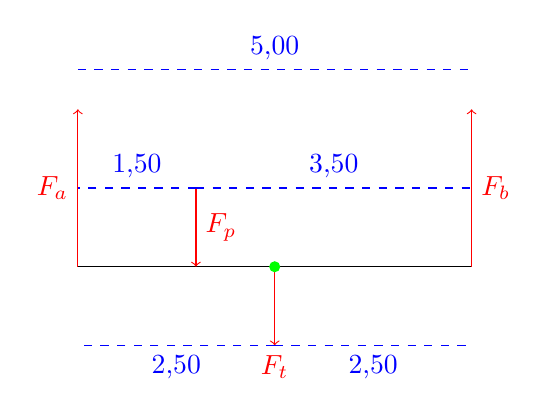
\begin{tikzpicture}
              \draw (-2.5,0) -- (2.5,0);


              \draw[->, red] (-2.5,1) ++(1.5,0) coordinate(fp) -- ++(0,-1) node[anchor=west,pos=.5]{$F_p$};
              \draw[->, red] (0,0) -- ++(0,-1)  coordinate(ft) node[anchor=north]{$F_t$};

              \draw[dashed, blue] (fp) -- (-2.5,1) node[blue,pos=.5,anchor=south]{\SI{1,50}{\meter}};
              \draw[dashed, blue] (fp) -- (2.5,1) node[blue,pos=.5,anchor=south]{\SI{3,50}{\meter}};

              \draw[dashed, blue] (ft) -- (-2.5,-1) node[blue,pos=.5,anchor=north]{\SI{2,50}{\meter}};
              \draw[dashed, blue] (ft) -- (2.5,-1) node[blue,pos=.5,anchor=north]{\SI{2,50}{\meter}};

              \draw[dashed, blue] (-2.5,2.5) -- (2.5,2.5) node[blue,pos=.5,anchor=south]{\SI{5,00}{\meter}};

              \fill[green] circle(2pt);

              \draw[->, red] (-2.5,0) -- ++(0,2) node[anchor=east,pos=.5]{$F_a$};
              \draw[->, red] (2.5,0) -- ++(0,2) node[anchor=west,pos=.5]{$F_b$};
            \end{tikzpicture}
          \end{center}

          \[
            F_p=\SI{75,0}{\kilogram}\times\SI{9,80}{\meter\over\second}
            =\SI{735}{\newton}
          \]
          \[
            F_t=\SI{15,0}{\kilogram}\times\SI{9,80}{\meter\over\second}
            =\SI{147}{\newton}
          \]
          \[
            F_a=-F_p\times\frac{\SI{3,50}{\meter}}{\SI{5,00}{\meter}}-F_t\times\frac{\SI{2,50}{\meter}}{\SI{5,00}{\meter}}
            =\boxed{\SI{-588}{\newton}}
          \]
          \[
            F_b=-F_p\times\frac{\SI{1,50}{\meter}}{\SI{5,00}{\meter}}-F_t\times\frac{\SI{2,50}{\meter}}{\SI{5,00}{\meter}}
            =\boxed{\SI{-294}{\newton}}
          \]
        \end{multicols}

        \newpage
  \item Despreciando las masas de las varillas horizontales y de las cuerdas y sabiendo que la abeja de la izquierda tiene una masa de \SI{0,100}{\kilogram}. ¿Cuál debe ser la masa de cada una de las otras figuras para que el móvil permanezca “equilibrado”?

        \begin{center}
          \begin{tikzpicture}
            \draw (1,0) -- ++(0,-2) coordinate(l1);
            \draw (l1) -- ++(-3,0) node[blue,pos=.5,anchor=south]{\SI{30,0}{\cm}} coordinate(l1a);
            \draw[red,->] (l1a) -- ++(0,-1) node[anchor=north]{$F_f$};
            \draw (l1) -- ++(1.5,0) node[blue,pos=.5,anchor=south]{\SI{15,0}{\cm}} coordinate(l1b);

            \draw (l1b) -- ++(0,-2) coordinate(l2);
            \draw (l2) -- ++(1.5,0) node[blue,pos=.5,anchor=south]{\SI{15,0}{\cm}} coordinate(l2b);
            \draw[red,->] (l2b) -- ++(0,-1) node[anchor=north]{$F_d$};
            \draw (l2) -- ++(-2.5,0) node[blue,pos=.5,anchor=south]{\SI{25,0}{\cm}} coordinate(l2a);

            \draw (l2a) -- ++(0,-2) coordinate(l3);
            \draw (l3) -- ++(2,0) node[blue,pos=.5,anchor=south]{\SI{20,0}{\cm}} coordinate(l3b);
            \draw[red,->] (l3b) -- ++(0,-1) node[anchor=north]{$F_b$};
            \draw (l3) -- ++(-4,0) node[blue,pos=.5,anchor=south]{\SI{40,0}{\cm}} coordinate(l3a);
            \draw[red,->] (l3a) -- ++(0,-1) node[anchor=north]{$F_a$};

            \fill[green] (l1) circle(2pt) (l2) circle(2pt) (l3) circle(2pt);

            \fill[cyan] (l1a) circle(2pt) node[anchor=south]{$M_f$} (l2b) circle(2pt) node[anchor=west]{$M_d$} (l3b) circle(2pt) node[anchor=south]{$M_b$} (l3a) circle(2pt) node[anchor=south]{$M_a$};

            \draw[red,dashed,->] (l2a) ++(-.2,0) -- ++ (0,-1) node[pos=.5,anchor=east]{$F_c$};
            \draw[red,dashed,->] (l1b) ++(.2,0) -- ++ (0,-1) node[pos=.5,anchor=west]{$F_e$};
          \end{tikzpicture}
        \end{center}

        \begin{multicols}{2}
          \[M_a=\SI{0,100}{\kilogram}\]
          \[
            F_a=M_a\times g
            =\SI{0,100}{\kilogram}\times\SI{9,80}{\meter\over\second}
            =\SI{0,980}{\newton}
          \]
          \[
            \tau_a=rF_a\sin{\theta}
            =\SI{40,0}{\cm}\times\SI{0,980}{\newton}\times\sin{\ang{90}}
            =\SI{39,2}{\newton\cm}
          \]
          \[\tau_b=-\tau_a\]
          \[rF_b\sin{\theta}=\SI{-39,2}{\newton\cm}\]
          \[\SI{20,0}{\cm}\times F_b\times\sin{\ang{-90}}=\SI{-39,2}{\newton\cm}\]
          \[\SI{-20,0}{\cm}\times F_b=\SI{-39,2}{\newton\cm}\]
          \[F_b=\SI{1.96}{\newton}\]
          \[
            M_b=\frac{F_b}{g}
            =\frac{\SI{1.96}{\newton}}{\SI{9,80}{\meter\over\second}}
            =\boxed{\SI{0,200}{\kilogram}}
          \]

          \[
            F_c=F_a+F_b
            =\SI{0,980}{\newton}+\SI{1.96}{\newton}
            =\SI{2,94}{\newton}
          \]
          \[
            \tau_c=rF_c\sin{\theta}
            =\SI{25,0}{\cm}\times\SI{2,94}{\newton}\times\sin{\ang{90}}
            =\SI{73,5}{\newton\cm}
          \]
          \[\tau_d=-\tau_c\]
          \[rF_d\sin{\theta}=\SI{-73,5}{\newton\cm}\]
          \[\SI{15,0}{\cm}\times F_d\times\sin{\ang{-90}}=\SI{-73,5}{\newton\cm}\]
          \[\SI{-15,0}{\cm}\times F_d=\SI{-73,5}{\newton\cm}\]
          \[F_d=\SI{4,90}{\newton}\]
          \[
            M_d=\frac{F_d}{g}
            =\frac{\SI{4,90}{\newton}}{\SI{9,80}{\meter\over\second}}
            =\boxed{\SI{0,500}{\kilogram}}
          \]

          \[
            F_e=F_c+F_d
            =\SI{2,94}{\newton}+\SI{4,90}{\newton}
            =\SI{7,84}{\newton}
          \]
          \[
            \tau_e=rF_e\sin{\theta}
            =\SI{15,0}{\cm}\times\SI{7,84}{\newton}\times\sin{\ang{-90}}
            =\SI{-117,6}{\newton\cm}
          \]
          \[\tau_f=-\tau_e\]
          \[rF_f\sin{\theta}=\SI{117,6}{\newton\cm}\]
          \[\SI{30,0}{\cm}\times F_d\times\sin{\ang{90}}=\SI{117,6}{\newton\cm}\]
          \[\SI{30,0}{\cm}\times F_d=\SI{117,6}{\newton\cm}\]
          \[F_f=\SI{3,92}{\newton}\]
          \[
            M_d=\frac{F_d}{g}
            =\frac{\SI{3,92}{\newton}}{\SI{9,80}{\meter\over\second}}
            =\boxed{\SI{0,400}{\kilogram}}
          \]
        \end{multicols}

        \newpage
  \item Se suspende una masa de dos cuerdas tal como se muestra en la figura. ¿Cuáles son las tensiones en las cuerdas?

        \begin{center}
          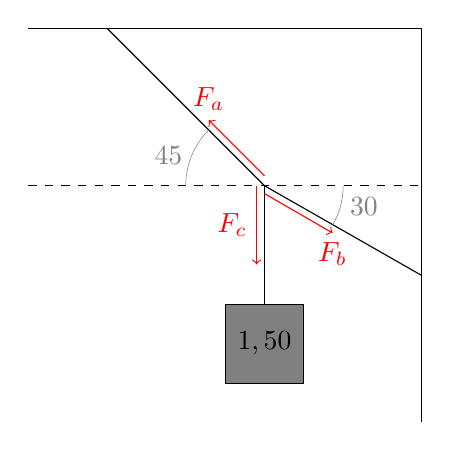
\begin{tikzpicture}
            \draw (-5,0) -- (0,0) -- (0,-5);
            \draw (-4,0) -- (-2,-2) coordinate(x) -- (0,-pi);
            \draw[dashed] (-5,-2) -- (0,-2);
            \draw[help lines] (x) ++(-30:1) arc(-30:0:1) node[pos=.5,anchor=west]{\ang{30}};
            \draw[help lines] (x) ++(135:1) arc(135:180:1) node[pos=.5,anchor=east]{\ang{45}};
            \draw (x) -- ++(0,-1.5) node[anchor=north,fill=gray,draw,minimum size=1cm]{$\SI{1,50}{\kilogram}$};

            \draw[red,->] (x) ++(0,.125) -- ++(135:1) node[anchor=south]{$F_a$};
            \draw[red,->] (x) ++(0,-.1) -- ++(-30:1) node[anchor=north]{$F_b$};
            \draw[red,->] (x) ++(-180:.1) -- ++(0,-1) node[pos=.5,anchor=east]{$F_c$};
          \end{tikzpicture}
        \end{center}

        \begin{multicols}{2}
          \[
            F_c=\SI{1,50}{\kilogram}\times\SI{9,80}{\meter\over\second}
            =\SI{14,7}{\newton}
          \]
          \[F_a+F_b+F_c=0\]

          \[F_{ax}+F_{bx}=0\]
          \[F_a\cos{\ang{135}}+F_b\cos{\ang{-30}}=0\]
          \[-F_a\cos{\ang{45}}+F_b\cos{\ang{30}}=0\]
          \[F_b\cos{\ang{30}}=F_a\cos{\ang{45}}\]
          \[F_b=F_a\frac{\cos{\ang{45}}}{\cos{\ang{30}}}\]

          \[F_{ay}+F_{by}+F_{cy}=0\]
          \[F_a\sin{\ang{135}}+F_b\sin{\ang{-30}}-\SI{14,7}{\newton}=0\]
          \[F_a\sin{\ang{45}}-F_a\cos{\ang{45}}\tan{\ang{30}}-\SI{14,7}{\newton}=0\]
          \[F_a\sin{\ang{45}}-F_a\cos{\ang{45}}\tan{\ang{30}}=\SI{14,7}{\newton}\]
          \[F_a(\sin{\ang{45}}-\cos{\ang{45}}\tan{\ang{30}})=\SI{14,7}{\newton}\]
          \[F_a=\frac{\SI{14,7}{\newton}}{\sin{\ang{45}}-\cos{\ang{45}}\tan{\ang{30}}}\]
          \[F_a=\boxed{\SI{49.2}{\newton}}\]

          \[F_b=\SI{49,2}{\newton}\frac{\cos{\ang{45}}}{\cos{\ang{30}}}\]
          \[F_b=\boxed{\SI{40,2}{\newton}}\]
        \end{multicols}

  \item Calcular que ángulo máximo puede formar con la vertical cada una de las cuatro cuerdas de la figura, para que la tensión que soporta cada una no exceda los \SI{500}{\newton}. (Use consideraciones de simetria)

        \begin{multicols}{2}
          \begin{center}
            \begin{tikzpicture}
              \draw (0,0) -- ++(3,0) -- ++(0,-2);
              \draw (-1,-1) -- ++(3,0) -- ++(0,-2) -- ++(-3,0) -- ++(0,2);
              \draw (0,0) -- ++(-1,-1) ++(3,0) -- ++(1,1) ++(0,-2) -- ++(-1,-1);

              \draw[red] (1,2) coordinate(a) node[anchor=south]{$F$};
              \draw[red] (0,0) -- (a) (3,0) -- (a) (-1,-1) -- (a) (2,-1) -- (a);

              \draw[dashed] (3,0) -- ++(0,2);
              \draw[help lines] (3,1) -- ++arc(90:135:1) node[pos=.5,anchor=south]{$\theta$};
            \end{tikzpicture}
          \end{center}

          \[F_y=\frac{\SI{1,00e3}{\newton}}{4}=\SI{250}{\newton}\]
          \[{F_x}^2+{F_y}^2=(\SI{500}{\newton})^2\]
          \[{F_x}^2+\SI{6,25e4}{\newton}=\SI{2,50e5}{\newton}\]
          \[{F_x}^2=\SI{1,87e5}{\newton}\]
          \[F_x=\SI{432}{\newton}\]
          \[\SI{500}{\newton}\times\cos{(\ang{90}-\theta)}=\SI{432}{\newton}\]
          \[\cos{(\ang{90}-\theta)}=\SI{0,864}{\newton}\]
          \[(\ang{90}-\theta)=\cos^{-1}{\SI{0,864}{\newton}}\]
          \[(\ang{90}-\theta)=\ang{30}\]
          \[\theta=\boxed{\ang{60}}\]
        \end{multicols}

  \item Una lámpara cuyo peso es $F_p$, está sostenida por dos cuerdas como muestra la figura. Si la tensión en la cuerda vale $F_p$, entonces los ángulos $\alpha$ y $\beta$ son respectivamente:

        \begin{multicols}{2}
          \begin{center}
            \begin{tikzpicture}
              \draw (-2.5,1) -- (2.5,1);
              \draw[red,->] (0,0) -- (150:2) coordinate(a) node[anchor=south]{$F_a$};
              \draw[help lines] (150:2) ++(1,0) -- ++arc(0:-30:1) node[pos=.5,anchor=west]{$\alpha$};
              \draw[red,->] (0,0) -- (30:2) coordinate(b) node[anchor=south]{$F_b$};
              \draw[help lines] (30:2) ++(-1,0) -- ++arc(180:210:1) node[pos=.5,anchor=east]{$\beta$};
              \draw[red,->] (0,0) -- (270:2) coordinate(c) node[anchor=north]{$F_p$};

              \draw[dashed,help lines] (a) -- (c) (b) -- (c);
            \end{tikzpicture}
          \end{center}

          \[F_a=F_b=F_p\]
          \[F_a=F_b\land F_{ax}+F_{bx}=0\implies\alpha=\beta\]

          Los vectores $F_A$, $F_b$, y $F_p$ son simetricos, y al tener los mismos angulos y magnitudes, sus puntas forman un triangulo equilatero, cuyos angulos internos solo pueden ser de \ang{60}. Ergo:

          \[\boxed{\alpha=\beta=\ang{30}}\]
        \end{multicols}

  \item Una revista especializada infoma que cierto auto deportivo tiene \num{53,0}\% de su peso en las ruedas delanteras y el \num{47,0}\% sobre las traseras, con una distancia entre ejes de $d=\SI{2,46}{\meter}$. Esto implica que la fuerza normal total sobre las ruedas delanteras es de $\num{0,530}P$ y sobre las traseras, de $\num{0,470}P$, donde $P$ es el peso total. Al espacio entre el eje delantero y trasero se llama distancia entre ejes. ¿Qué tan adelante del eje trasero esta el centro de gravedad del automóvil?

        \begin{multicols}{2}
          \begin{center}
            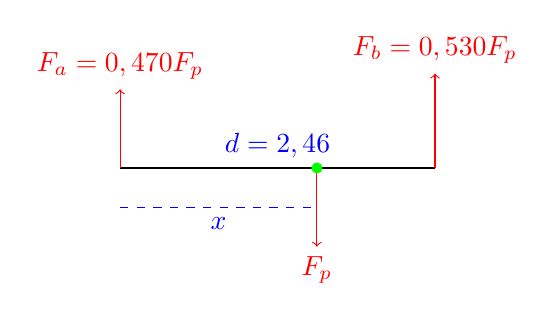
\begin{tikzpicture}
              \draw (0,0) -- (4,0) node[pos=.5,anchor=south,blue]{$d=\SI{2,46}{\meter}$};
              \draw[red,->] (0,0) -- ++(0,1) node[anchor=south]{$F_a=\num{0,470}F_p$};
              \draw[red,->] (4,0) -- ++(0,1.2) node[anchor=south]{$F_b=\num{0,530}F_p$};

              \draw[red,->] (2.5,0) -- ++(0,-1) node[anchor=north]{$F_p$};
              \draw[blue,dashed] (0,-.5) -- (2.5,-.5) node[pos=.5,anchor=north]{$x$};
              \fill[green] (2.5,0) circle(2pt);
            \end{tikzpicture}
          \end{center}

          \[F_b=F_p\times\frac{x}{d}\]
          \[\num{0,530}F_p=F_p\times\frac{x}{\SI{2,46}{\meter}}\]
          \[\num{0,530}=\frac{x}{\SI{2,46}{\meter}}\]
          \[\num{0,530}\times\SI{2,46}{\meter}=x\]
          \[x=\boxed{\SI{1,30}{\meter}}\]
        \end{multicols}

        \newpage
  \item Una grúa torre como muestra la figura, debe siempre estar cuidadosamente balanceada de manera que no haya un torque (o momento) neto que tienda a voltearla. Una grúa está a punto de levantar una carga de \SI{2,80e3}{\kilogram}. Las dimensiones de la grúa se muestran en la figura. Ignore la masa de la viga horizontal.

        \begin{center}
          \begin{tikzpicture}
            \draw (0,0) -- ++(0,3) coordinate(center) -- ++(0,1);
            \draw (center) -- ++(-3,0) node[pos=.5,anchor=north,blue]{\SI{3,40}{\meter}};
            \draw[red,->] (center) ++(-2.5,0) -- ++(0,-1) node[anchor=north]{$F_a$};
            \draw[blue,dashed] (center) ++(0,.5) -- ++(-2.5,0) node[pos=.5,anchor=south]{$x$};
            \draw (center) -- ++(4,0) coordinate(weight) node[pos=.5,anchor=north,blue]{\SI{7,70}{\meter}};
            \draw[red,->] (weight) -- ++(0,-1) node[anchor=north]{$F_b$};
            \fill[green] (center) circle(2pt);
          \end{tikzpicture}
        \end{center}

        \begin{enumerate}
          \item Dónde debe colocarsse el contrapeso de \SI{9,50e3}{\kilogram} cuando la carga se levanta desde el suelo?

                \[
                  F_a=\SI{9,50e3}{\kilogram}\times\SI{9,80}{\meter\over\second\squared}
                  =\SI{9,31e4}{\newton}
                \]
                \[
                  F_b=\SI{2,80e3}{\kilogram}\times\SI{9,80}{\meter\over\second\squared}
                  =\SI{2,74e4}{\newton}
                \]
                \[
                  \tau_b=rF_b\sin{\theta}
                  =\SI{7,70}{\meter}\times\SI{2,74e4}{\newton}\times\sin{\ang{-90}}
                  =\SI{-2,11e5}{\newton\meter}
                \]

                \[\tau_a=-\tau_b=rF_a\sin{\theta}\]
                \[\SI{2,11e5}{\newton\meter}=x\times\SI{9,31e4}{\newton}\times\sin{\ang{90}}\]
                \[\frac{\SI{2,11e5}{\newton\meter}}{\SI{9,31e4}{\newton}}=x\]
                \[x=\boxed{\SI{2,27}{\meter}}\]

          \item Determine la carga máxima que puede ser levantada cuando el contrapeso se coloca en el punto extremo de la grúa.

                \[
                  \tau_a=rF_a\sin{\theta}
                  =\SI{3,40}{\meter}\times\SI{9,31e4}{\newton}\times\sin{\ang{90}}
                  =\SI{3,17e5}{\meter\newton}
                \]

                \[\tau_b=-\tau_a=rF_b\sin{\theta}\]
                \[\SI{-3,17e5}{\meter\newton}=\SI{7,70}{\meter}\times F_b\times\sin{\ang{-90}}\]
                \[\frac{\SI{-3,17e5}{\meter\newton}}{\SI{-7,70}{\meter}}=F_b\]
                \[F_b=\SI{4,17e4}{\newton}\]

                \[
                  M=\frac{F_b}{g}
                  =\frac{\SI{4,17e4}{\newton}}{\SI{9,80}{\meter\over\second\squared}}
                  =\boxed{\SI{4,26e3}{\kilogram}}
                \]
        \end{enumerate}
\end{enumerate}
\end{document}
